%%
% 第二章：系统设计与实现
%%

\chapter{系统设计与实现}
\label{chap:design}

\section{设计目标与总体流程}

PathTracer 要做的事情很简单：给定一个 Python 源文件，找出其中有哪些控制结构，在程序运行时记录实际执行路径，最后把两类信息合并成覆盖率报告。本章直接结合核心代码说明各模块是怎样工作的。

整个系统分四步。第一步，命令行接口读取用户参数，确定目标文件、输出格式和传给目标程序的参数。第二步，静态分析器扫描源文件，抽取 \texttt{if}、\texttt{for}、\texttt{while} 和 \texttt{except} 等控制结构。第三步，运行时追踪器利用 \texttt{sys.settrace} 记录目标文件中实际执行过的代码行，并顺带构造函数调用树。第四步，报告生成器把静态结构和动态执行位置对齐，输出文本、JSON 或 HTML 报告。

\begin{figure}[htbp]
    \centering
    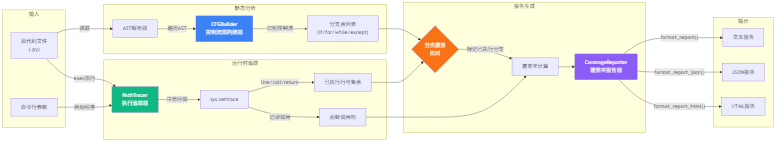
\includegraphics[width=0.95\textwidth]{figures/pathtracer-architecture.png}
    \caption{PathTracer 系统架构图}
    \label{fig:architecture}
\end{figure}

每个模块只做一件事：静态分析器不管程序怎么运行，追踪器不管代码里有多少控制结构，报告生成器只负责汇总。模块之间靠统一的数据结构传值，互相不依赖内部实现。

\section{模块划分与调用关系}

PathTracer 的源码集中在 \path{pathtracer} 目录下，核心模块有五个。\path{models.py} 定义统一的数据结构，在模块之间传递分支、执行路径和报告数据。\path{tracer.py} 实现运行时追踪，记录执行行号和函数调用信息。\path{cfg_builder.py} 实现静态分析，从抽象语法树中提取控制结构。\path{reporter.py} 把静态结果和动态结果合并成覆盖率报告。\path{cli.py} 提供命令行入口，调度前面四个模块。

调用关系是线性的。命令行入口先创建 \texttt{PathTracer} 实例，再执行目标程序；程序运行结束后，\texttt{CoverageReporter} 调用 \texttt{CFGBuilder} 获取静态分支集合，同时从追踪器中取出执行行集合；最后将命中结果写回 \texttt{CoverageReport}。\texttt{models.py} 定义公共数据格式，其他模块围绕这些结构顺次工作。

\section{数据模型设计}

先把数据结构定下来，后面各模块的代码就好写了。下面这段代码来自 \path{pathtracer/models.py}：

\begin{lstlisting}[language=Python, caption={PathTracer 的核心数据模型}]
from dataclasses import dataclass, field
from typing import Set, Dict, List, Optional
from enum import Enum


class BranchType(Enum):
    # 统一定义可统计的控制结构类型
    SEQUENTIAL = "sequential"
    IF = "if"
    ELSE = "else"
    ELIF = "elif"
    FOR = "for"
    WHILE = "while"
    TRY = "try"
    EXCEPT = "except"


@dataclass
class CodeBranch:
    # 表示源码中的一个静态控制结构入口
    file_path: str
    line_no: int
    branch_type: BranchType
    end_line: int = 0
    is_executed: bool = False


@dataclass
class ExecutionPath:
    # 保存一次运行中某个文件的动态执行结果
    file_path: str
    executed_lines: Set[int] = field(default_factory=set)
    executed_branches: Dict[int, CodeBranch] = field(
        default_factory=dict
    )
    function_calls: List["FunctionCall"] = field(
        default_factory=list
    )


@dataclass
class CoverageReport:
    # 汇总最终统计结果，供文本/JSON/HTML 三种报告复用
    total_branches: int = 0
    executed_branches: int = 0
    branches_by_type: Dict[BranchType, int] = field(
        default_factory=dict
    )
    coverage_percentage: float = 0.0
    file_reports: Dict[str, ExecutionPath] = field(
        default_factory=dict
    )
\end{lstlisting}

\texttt{BranchType} 统一描述控制结构类型，\texttt{CodeBranch} 表示源代码中的静态分支点，\texttt{ExecutionPath} 记录某个文件在一次运行中的动态执行结果，\texttt{CoverageReport} 汇总最终统计。各模块之间不需要靠零散字典传值，始终围绕同一套结构工作。

\texttt{BranchType} 的定义比当前实现更宽。枚举里预留了 \texttt{SEQUENTIAL}、\texttt{ELSE}、\texttt{ELIF} 和 \texttt{TRY} 等类型，但静态提取器还没有全部识别。数据模型给后续扩展留了空间，识别能力可以继续补齐。

\texttt{CodeBranch} 和 \texttt{ExecutionPath} 是最关键的一对：前者描述"代码里有哪些结构"，后者描述"这次运行走了哪些位置"。报告生成器做的事，就是把这两份信息对齐。

\section{运行时追踪器实现}

\texttt{PathTracer} 是系统的动态部分，借助 \texttt{sys.settrace} 注册回调函数，在解释器执行目标程序时实时接收事件。核心实现如下：

\begin{lstlisting}[language=Python, caption={运行时追踪器的核心回调逻辑}]
class PathTracer:
    def __init__(self):
        # 每个目标文件对应一份独立的执行记录
        self.execution_paths = {}
        self._original_trace = None
        self._target_file = None
        self.function_calls = []
        self._call_stack = []

    def trace_file(self, file_path: str) -> "PathTracer":
        # 指定本次要追踪的目标文件，并预先创建容器
        self._target_file = file_path
        self.execution_paths[file_path] = ExecutionPath(
            file_path=file_path
        )
        return self

    def _trace_callback(self, frame, event: str, arg):
        if not self._target_file:
            return None

        code = frame.f_code
        # 只保留目标文件中的事件，过滤掉标准库和第三方库
        if not code.co_filename.endswith(self._target_file):
            return self._trace_callback

        if event == "line":
            # line 事件只记录"哪一行被执行到了"
            line_no = frame.f_lineno
            path = self.execution_paths[self._target_file]
            path.executed_lines.add(line_no)

        elif event == "call":
            # call 事件额外记录函数名、参数和调用层级
            func_name = code.co_name
            line_no = frame.f_lineno
            args = {}
            arg_count = code.co_argcount
            arg_names = code.co_varnames[:arg_count]
            for arg_name in arg_names:
                if arg_name in frame.f_locals:
                    args[arg_name] = repr(frame.f_locals[arg_name])

            call_depth = len(self._call_stack)
            func_call = FunctionCall(
                function_name=func_name,
                file_path=code.co_filename,
                line_no=line_no,
                call_depth=call_depth,
                arguments=args,
            )

            if self._call_stack:
                # 若当前已有父调用，则把它挂到父节点下面
                self._call_stack[-1].children.append(func_call)
            else:
                # 否则它就是一棵调用树的根节点
                self.function_calls.append(func_call)
                path = self.execution_paths[self._target_file]
                path.function_calls.append(func_call)
            self._call_stack.append(func_call)

        elif event == "return":
            # return 事件与最近一次 call 配对，用于补全返回值
            if self._call_stack:
                func_call = self._call_stack.pop()
                if arg is not None:
                    func_call.return_value = repr(arg)

        return self._trace_callback
\end{lstlisting}

这段代码有几个实现细节值得单独说。

\texttt{trace\_file()} 并不直接启动追踪。它先保存目标文件路径，再初始化对应的 \texttt{ExecutionPath}，后面回调函数就能把结果直接写入固定位置。

\path{code.co_filename.endswith(self._target_file)} 限制了追踪范围，只记录目标文件中的事件，不把标准库、第三方库甚至 PathTracer 自身的内部调用算进去。不做这个过滤，输出会被大量无关代码淹没。

\texttt{line} 事件和 \texttt{call}/\texttt{return} 事件被分开处理。前者只记录哪些行被执行过；后者负责构造函数调用树。覆盖率统计和调用树展示都来自同一个回调，但在数据层面是分开的。

函数调用树靠 \texttt{\_call\_stack} 维护层级。每次 \texttt{call} 事件把新的 \texttt{FunctionCall} 压栈，\texttt{return} 事件弹出并补上返回值。这个栈结构是调用树能够成立的基础。

追踪器还实现了上下文管理器接口：

\begin{lstlisting}[language=Python, caption={追踪器的启停方式}]
def __enter__(self):
    # 保存原来的追踪状态，避免影响外部环境
    self._original_trace = sys.gettrace()
    sys.settrace(self._trace_callback)
    return self


def __exit__(self, exc_type, exc_val, exc_tb):
    # 退出时恢复原来的追踪函数
    sys.settrace(self._original_trace)
    return False
\end{lstlisting}

进入 \texttt{with} 块时注册追踪函数，退出时恢复原来的状态。PathTracer 的启停成对出现，外部调用简洁。

\section{静态分支提取实现}

动态追踪只能告诉我们"程序执行到了哪里"，但不知道"代码里一共有多少个控制结构"。这部分由 \texttt{CFGBuilder} 完成。它没有真的去构建控制流图，而是用 AST 扫描出需要统计的控制结构入口：

\begin{lstlisting}[language=Python, caption={基于 AST 的静态分支提取}]
class CFGBuilder:
    def build_from_file(self, file_path: str):
        # 先读源码，再交给 ast 构建语法树
        with open(file_path, "r", encoding="utf-8") as f:
            source = f.read()

        tree = ast.parse(source, filename=file_path)
        self.branches = []

        for node in ast.walk(tree):
            # 逐个检查 AST 节点，筛出需要统计的控制结构
            branch = self._extract_branch(file_path, node)
            if branch:
                self.branches.append(branch)

        return self.branches

    def _extract_branch(self, file_path: str, node: ast.AST):
        if isinstance(node, ast.If):
            # 记录 if 结构入口及其代码范围
            return CodeBranch(
                file_path=file_path,
                line_no=node.lineno,
                branch_type=BranchType.IF,
                end_line=self._get_end_line(node),
            )
        elif isinstance(node, ast.For):
            # 记录 for 循环入口
            return CodeBranch(
                file_path=file_path,
                line_no=node.lineno,
                branch_type=BranchType.FOR,
                end_line=self._get_end_line(node),
            )
        elif isinstance(node, ast.While):
            # 记录 while 循环入口
            return CodeBranch(
                file_path=file_path,
                line_no=node.lineno,
                branch_type=BranchType.WHILE,
                end_line=self._get_end_line(node),
            )
        elif isinstance(node, ast.ExceptHandler):
            # 记录 except 处理分支
            return CodeBranch(
                file_path=file_path,
                line_no=node.lineno,
                branch_type=BranchType.EXCEPT,
                end_line=self._get_end_line(node),
            )

        return None
\end{lstlisting}

实现思路是用 \texttt{ast.parse} 把源码转成抽象语法树，再用 \texttt{ast.walk} 遍历所有节点，只保留控制结构相关的几类。每发现一个目标节点，就创建一个 \texttt{CodeBranch} 对象。

有两个设计取舍。第一，当前只统计 \texttt{if}、\texttt{for}、\texttt{while} 和 \texttt{except}，没有覆盖 \texttt{with}、\texttt{match-case} 或异步语法。第二，统计的是"结构入口"而不是"结构方向"。例如 \texttt{if} 语句被记成一个分支点，但不会细分真分支和假分支。所以本文更准确的说法是"控制结构命中率"。

另一个细节是为每个结构记录结束行号：

\begin{lstlisting}[language=Python, caption={控制结构结束行号的计算}]
def _get_end_line(self, node: ast.AST) -> int:
    # Python 3.8+ 优先直接使用 AST 节点的结束行号
    if hasattr(node, "end_lineno") and node.end_lineno is not None:
        return node.end_lineno
    # 若没有 end_lineno，就递归取 body 中最靠后的行号
    if hasattr(node, "body") and node.body:
        return max(self._get_end_line(n) for n in node.body)
    # 再退一步，就把起始行号当作结束行号
    return getattr(node, "lineno", 0)
\end{lstlisting}

这个字段对命中判定不是必需的，但对报告展示有帮助。在 HTML 或 JSON 报告里，知道一个控制结构覆盖了哪一段代码，比只知道起始行号直观得多。

\section{覆盖率分析与报告生成}

静态分支和动态执行路径准备好之后，\texttt{CoverageReporter} 计算覆盖率。核心分析逻辑如下：

\begin{lstlisting}[language=Python, caption={覆盖率统计的核心实现}]
class CoverageReporter:
    def __init__(self):
        self.cfg_builder = CFGBuilder()

    def analyze(self, file_path: str, tracer: PathTracer) -> CoverageReport:
        # 静态部分：先找出该文件里所有可统计的控制结构
        all_branches = self.cfg_builder.build_from_file(file_path)
        # 动态部分：再取出本次运行真正命中的代码行
        executed_lines = tracer.get_executed_lines(file_path)

        for branch in all_branches:
            # 若控制结构起始行被执行到，则认为该结构被命中
            if branch.line_no in executed_lines:
                branch.is_executed = True

        total = len(all_branches)
        executed = sum(1 for b in all_branches if b.is_executed)

        by_type = {}
        for branch_type in BranchType:
            # 统计每类控制结构在源码中一共出现了多少次
            type_branches = [
                b for b in all_branches if b.branch_type == branch_type
            ]
            by_type[branch_type] = len(type_branches)

        return CoverageReport(
            total_branches=total,
            executed_branches=executed,
            branches_by_type=by_type,
            coverage_percentage=(
                (executed / total * 100) if total > 0 else 0.0
            ),
            file_reports={
                file_path: ExecutionPath(
                    file_path=file_path,
                    executed_lines=executed_lines,
                    # 只把已命中的结构写进最终报告
                    executed_branches={
                        b.line_no: b for b in all_branches if b.is_executed
                    },
                )
            },
        )
\end{lstlisting}

判断规则：某个控制结构的入口行号出现在执行行集合里，就标记为已执行。源码里对应 \path{branch.line_no in executed_lines}。这个规则不复杂，但和前面静态模块的"入口统计"口径一致。

统计完成后，报告生成器把结果转成不同格式。文本输出适合终端或论文正文；JSON 适合实验留档和后处理；HTML 偏可视化展示。下面是 JSON 报告的组织方式：

\begin{lstlisting}[language=Python, caption={JSON 报告的组织方式}]
def format_report_json(self, report: CoverageReport) -> str:
    # 先组织顶层统计字段
    data = {
        "coverage_percentage": report.coverage_percentage,
        "total_branches": report.total_branches,
        "executed_branches": report.executed_branches,
        "branches_by_type": {
            bt.value: count for bt, count in report.branches_by_type.items()
        },
        "file_reports": {},
        "function_calls": [],
    }

    for file_path, exec_path in report.file_reports.items():
        # 再逐文件补充执行行和已命中的结构列表
        file_data = {
            "executed_lines": sorted(
                list(exec_path.executed_lines)
            ),
            "executed_branches": [],
        }
        for _, branch in sorted(exec_path.executed_branches.items()):
            file_data["executed_branches"].append(
                {
                    "line_no": branch.line_no,
                    "branch_type": branch.branch_type.value,
                    "end_line": branch.end_line,
                }
            )
        data["file_reports"][file_path] = file_data

    # 最后序列化为 JSON 字符串
    return json.dumps(data, indent=2)
\end{lstlisting}

报告不只是输出一个覆盖率百分比。执行行集合、已命中分支列表和函数调用树都保留了，第三章可以直接引用结果文件展开分析。

不过当前实现有一个没完全打通的地方。\texttt{PathTracer} 在运行时已经记录了 \texttt{function\_calls}，但 \texttt{analyze()} 重建 \texttt{ExecutionPath} 时只写入了执行行和已命中分支，没有把函数调用树带入报告对象。JSON 和 HTML 侧预留了调用树的序列化与展示逻辑，但当前版本里这部分没有贯通到最终报告。

\section{命令行接口与执行流程}

前面几个模块分散手动调用并不方便。\texttt{cli.py} 把"解析参数、运行目标程序、触发分析、输出报告"这一整套流程串起来。核心代码如下：

\begin{lstlisting}[language=Python, caption={命令行入口的执行流程}]
def main():
    # 原始参数既包含 PathTracer 自己的选项，也包含目标程序参数
    raw_argv = sys.argv[1:]
    cli_argv = []
    program_args = []

    index = 0
    while index < len(raw_argv):
        arg = raw_argv[index]
        if arg in ("--output", "-o", "--format", "-f"):
            # 这些参数属于追踪器自身
            cli_argv.extend([arg, raw_argv[index + 1]])
            index += 2
            continue
        if arg in ("--quiet", "-q"):
            cli_argv.append(arg)
            index += 1
            continue
        # 第一个非追踪器参数视为目标脚本，剩余参数转交给它
        cli_argv.append(arg)
        program_args = raw_argv[index + 1:]
        break

    args = parser.parse_args(cli_argv)
    tracer = PathTracer().trace_file(args.program)
    reporter = CoverageReporter()

    try:
        # 重写 sys.argv，让目标脚本像平常一样读取命令行参数
        sys.argv = [args.program] + program_args
        with tracer:
            with open(args.program) as f:
                # 在当前进程里执行目标脚本，才能被 sys.settrace 捕获
                code = compile(f.read(), args.program, "exec")
                exec(
                    code,
                    {"__name__": "__main__", "__file__": args.program},
                )
    finally:
        # 目标脚本结束后立即生成报告
        report = reporter.analyze(args.program, tracer)
\end{lstlisting}

命令行参数被分成两部分：一部分属于 PathTracer 自己（输出格式、输出文件路径、静默模式），另一部分属于被测程序。通过手动扫描 \texttt{raw\_argv} 把两类参数拆开，避免追踪器自己的参数被错误传给目标脚本。

目标程序不是通过导入模块调用，而是通过 \texttt{compile + exec} 在当前进程里执行。只有目标脚本和追踪器处在同一个 Python 进程里，\texttt{sys.settrace} 才能捕获执行事件。

\section{与 PageIndex 的接入方式}

有了命令行入口，PathTracer 接入 PageIndex 很直接。把 \path{agent_pageindex.py} 作为目标文件，再把查询参数追加到命令后面即可：

\begin{lstlisting}[language=bash, caption={PathTracer 接入 PageIndex 的方式}]
python -m pathtracer.cli -f json -o docs/coverage_tc2.json \
    agent_pageindex.py -- --query "test" --verbose
\end{lstlisting}

PathTracer 不需要修改 PageIndex 的业务代码，也不需要给入口脚本打补丁。它在目标脚本运行前挂上追踪回调，在脚本结束后做一次静态分析和结果汇总。接入方式侵入性很低，不会影响被测项目原本的执行逻辑，实验结果也更接近真实使用场景。
